\subsection{Pride and Prejudice (Austen, 1813)}

\begin{figure}[H]\centering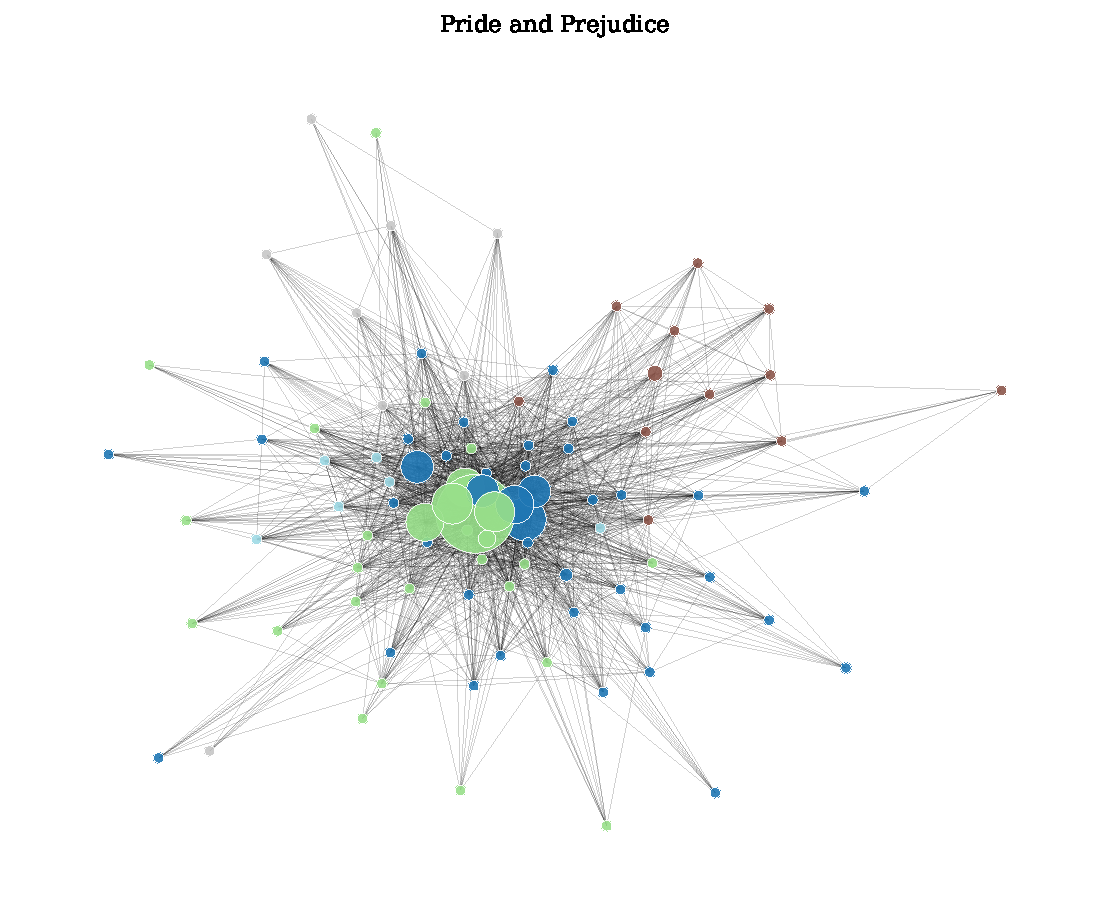
\includegraphics[width=0.74\textwidth]{figures/net_pride-and-prejudice.pdf}\caption{Character co-occurrence network of \emph{Pride and Prejudice}. Node size is proportional to betweenness and colours denote communities (greedy modularity); the most central characters are named in the accompanying table.}\end{figure}

\begin{table}[H]\centering\small
\begin{tabular}{lrrrr}
\toprule
Character & $C_B$ & Degree & Closeness & Eigenvector \\
\midrule
Elizabeth & 0.876 & 89 & 27.15 & 0.488 \\
Lydia & 0.072 & 83 & 26.27 & 0.245 \\
Mr. Darcy & 0.058 & 85 & 26.64 & 0.352 \\
Jane & 0.053 & 86 & 26.63 & 0.357 \\
Mrs. Bennet & 0.044 & 86 & 26.26 & 0.268 \\
Mr. Bingley & 0.043 & 78 & 26.18 & 0.252 \\
Miss Bingley & 0.042 & 62 & 25.60 & 0.149 \\
Lady Catherine & 0.022 & 74 & 26.22 & 0.255 \\
Sir William & 0.022 & 57 & 23.62 & 0.077 \\
Mr. Bennet & 0.021 & 75 & 25.57 & 0.175 \\
\bottomrule
\end{tabular}
\caption{Top-10 characters in \emph{Pride and Prejudice} ranked by betweenness.}\end{table}
\clearpage

\subsection{Moby-Dick (Melville, 1851)}

\begin{figure}[H]\centering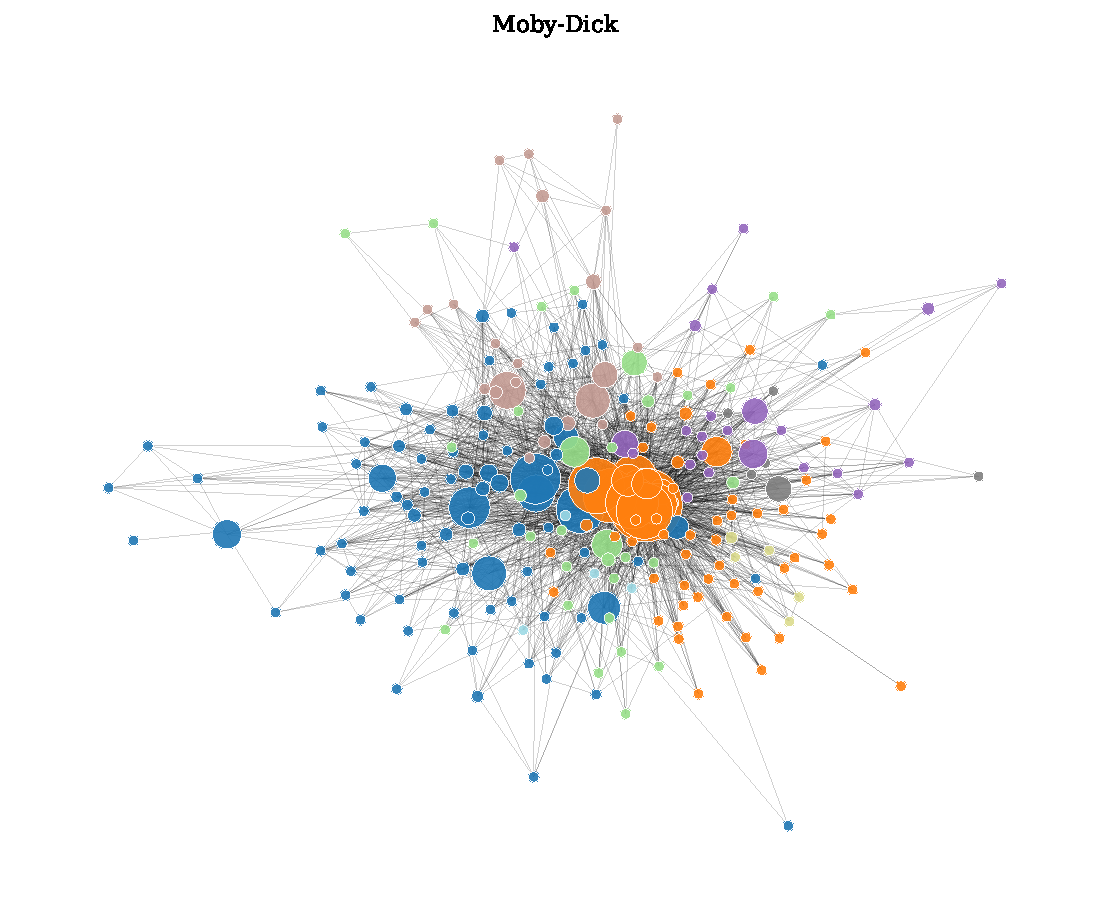
\includegraphics[width=0.74\textwidth]{figures/net_moby-dick.pdf}\caption{Character co-occurrence network of \emph{Moby-Dick}. Node size is proportional to betweenness and colours denote communities (greedy modularity); the most central characters are named in the accompanying table.}\end{figure}

\begin{table}[H]\centering\small
\begin{tabular}{lrrrr}
\toprule
Character & $C_B$ & Degree & Closeness & Eigenvector \\
\midrule
Ahab & 0.663 & 165 & 10.36 & 0.490 \\
Stubb (\#771) & 0.224 & 141 & 10.25 & 0.416 \\
God & 0.220 & 134 & 10.13 & 0.195 \\
Queequeg & 0.191 & 125 & 10.02 & 0.227 \\
the Pequod & 0.172 & 156 & 10.22 & 0.322 \\
Leviathan & 0.142 & 101 & 8.76 & 0.040 \\
the Sperm Whale & 0.115 & 90 & 9.55 & 0.089 \\
Moby Dick & 0.086 & 88 & 10.04 & 0.213 \\
Starbuck & 0.060 & 112 & 10.23 & 0.403 \\
Jonah & 0.060 & 65 & 8.03 & 0.012 \\
\bottomrule
\end{tabular}
\caption{Top-10 characters in \emph{Moby-Dick} ranked by betweenness.}\end{table}
\clearpage

\subsection{Frankenstein (Shelley, 1818)}

\begin{figure}[H]\centering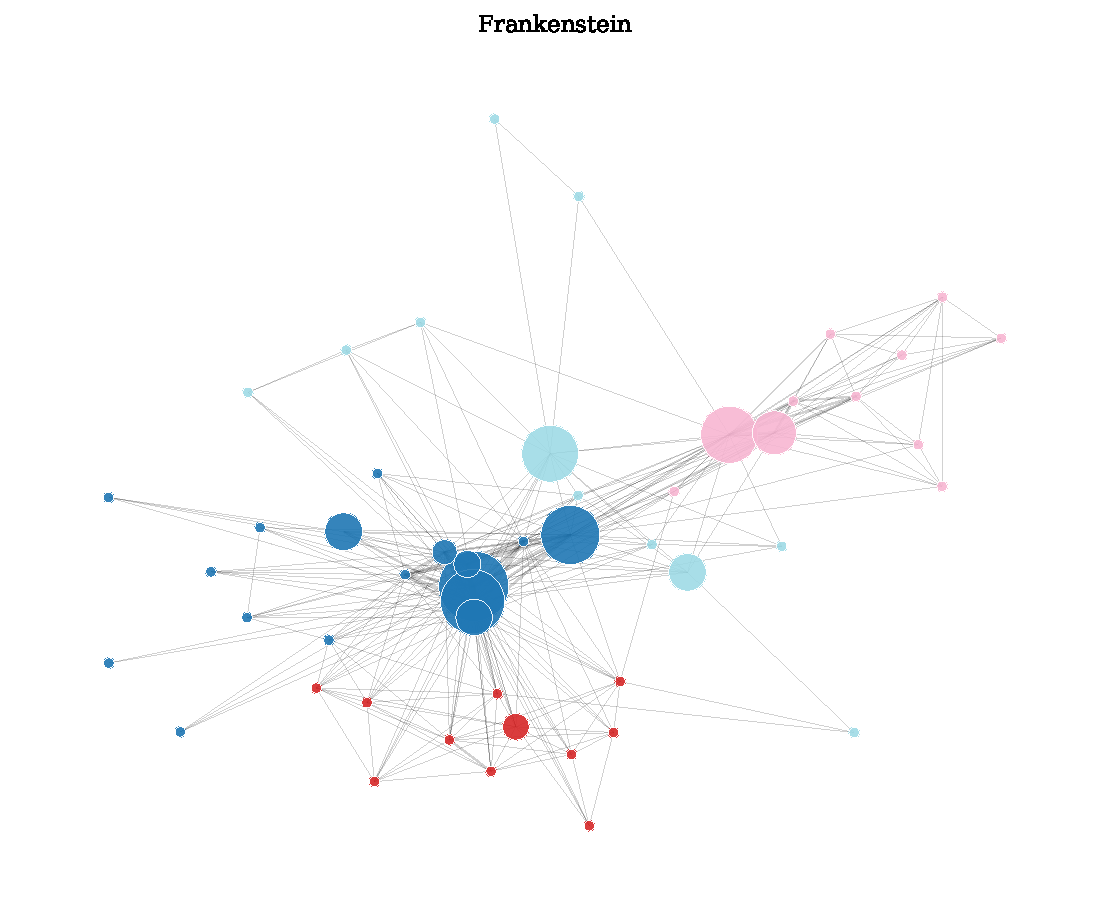
\includegraphics[width=0.74\textwidth]{figures/net_frankenstein.pdf}\caption{Character co-occurrence network of \emph{Frankenstein}. Node size is proportional to betweenness and colours denote communities (greedy modularity); the most central characters are named in the accompanying table.}\end{figure}

\begin{table}[H]\centering\small
\begin{tabular}{lrrrr}
\toprule
Character & $C_B$ & Degree & Closeness & Eigenvector \\
\midrule
Elizabeth & 0.550 & 36 & 9.66 & 0.507 \\
Clerval & 0.380 & 36 & 9.43 & 0.402 \\
God & 0.271 & 24 & 9.11 & 0.257 \\
Felix & 0.240 & 23 & 6.79 & 0.050 \\
Frankenstein (\#151) & 0.233 & 17 & 8.39 & 0.096 \\
Safie & 0.079 & 18 & 6.32 & 0.035 \\
Mr. Kirwin & 0.041 & 8 & 7.34 & 0.077 \\
Margaret & 0.040 & 11 & 5.96 & 0.039 \\
Victor & 0.035 & 26 & 9.03 & 0.352 \\
William & 0.009 & 26 & 8.96 & 0.366 \\
\bottomrule
\end{tabular}
\caption{Top-10 characters in \emph{Frankenstein} ranked by betweenness.}\end{table}
\clearpage

\subsection{A Tale of Two Cities (Dickens, 1859)}

\begin{figure}[H]\centering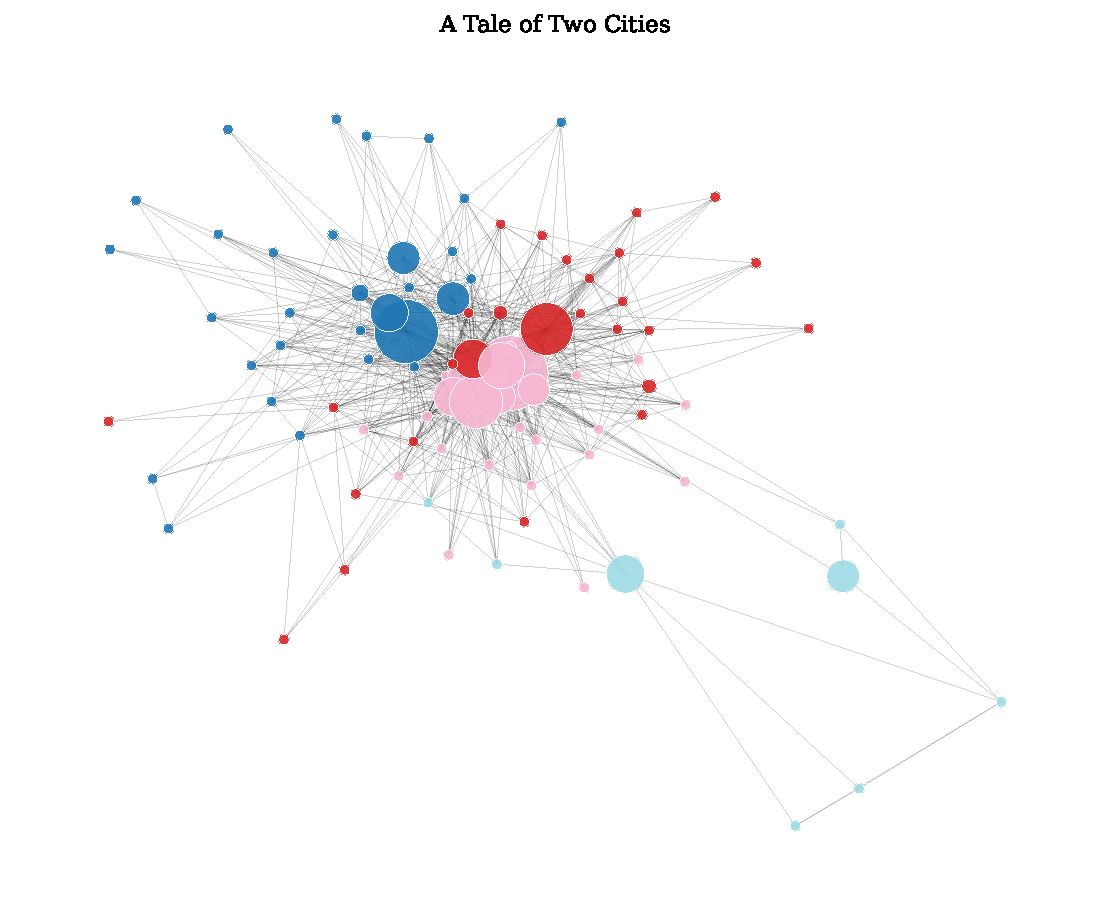
\includegraphics[width=0.74\textwidth]{figures/net_a-tale-of-two-cities.pdf}\caption{Character co-occurrence network of \emph{A Tale of Two Cities}. Node size is proportional to betweenness and colours denote communities (greedy modularity); the most central characters are named in the accompanying table.}\end{figure}

\begin{table}[H]\centering\small
\begin{tabular}{lrrrr}
\toprule
Character & $C_B$ & Degree & Closeness & Eigenvector \\
\midrule
Mr. Lorry & 0.695 & 60 & 15.11 & 0.468 \\
Madame Defarge & 0.382 & 48 & 14.45 & 0.215 \\
Darnay & 0.282 & 55 & 14.78 & 0.404 \\
Lucie & 0.179 & 47 & 14.60 & 0.356 \\
Mr. Cruncher & 0.171 & 46 & 13.62 & 0.126 \\
Miss Pross & 0.100 & 41 & 14.48 & 0.278 \\
Carton & 0.050 & 46 & 13.74 & 0.237 \\
Doctor Manette & 0.047 & 47 & 14.48 & 0.328 \\
Death & 0.044 & 11 & 5.43 & 0.007 \\
Saint Antoine & 0.043 & 36 & 12.96 & 0.062 \\
\bottomrule
\end{tabular}
\caption{Top-10 characters in \emph{A Tale of Two Cities} ranked by betweenness.}\end{table}
\clearpage

\subsection{Dracula (Stoker, 1897)}

\begin{figure}[H]\centering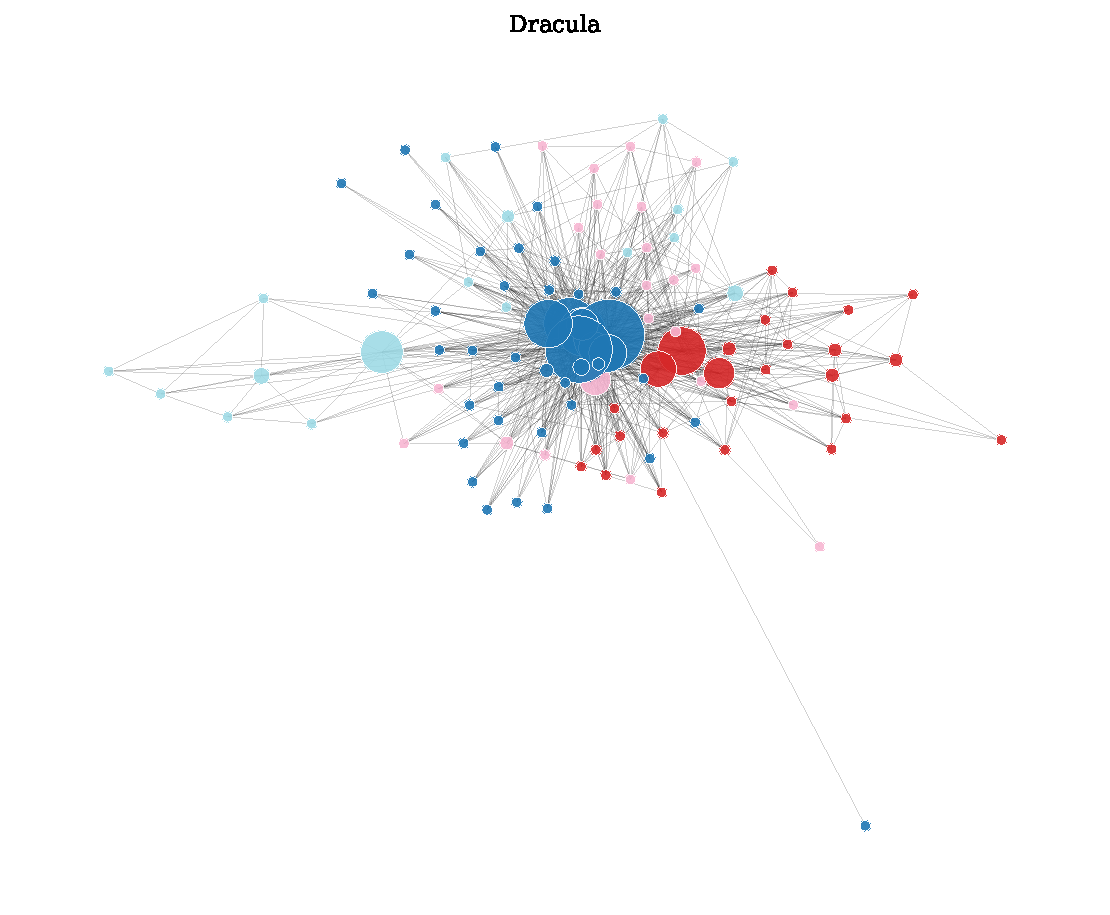
\includegraphics[width=0.74\textwidth]{figures/net_dracula.pdf}\caption{Character co-occurrence network of \emph{Dracula}. Node size is proportional to betweenness and colours denote communities (greedy modularity); the most central characters are named in the accompanying table.}\end{figure}

\begin{table}[H]\centering\small
\begin{tabular}{lrrrr}
\toprule
Character & $C_B$ & Degree & Closeness & Eigenvector \\
\midrule
Jonathan & 0.589 & 98 & 12.92 & 0.440 \\
Van Helsing (\#335) & 0.461 & 86 & 12.89 & 0.461 \\
Lucy & 0.162 & 76 & 12.78 & 0.361 \\
Renfield & 0.119 & 50 & 12.11 & 0.123 \\
Count Dracula & 0.118 & 46 & 11.47 & 0.047 \\
Dr. Seward & 0.116 & 88 & 12.77 & 0.347 \\
Lor & 0.069 & 21 & 6.97 & 0.007 \\
Lord Godalming & 0.042 & 63 & 12.60 & 0.247 \\
Galatz & 0.035 & 35 & 10.95 & 0.048 \\
Arthur & 0.019 & 69 & 12.63 & 0.300 \\
\bottomrule
\end{tabular}
\caption{Top-10 characters in \emph{Dracula} ranked by betweenness.}\end{table}
\clearpage

\subsection{Great Expectations (Dickens, 1861)}

\begin{figure}[H]\centering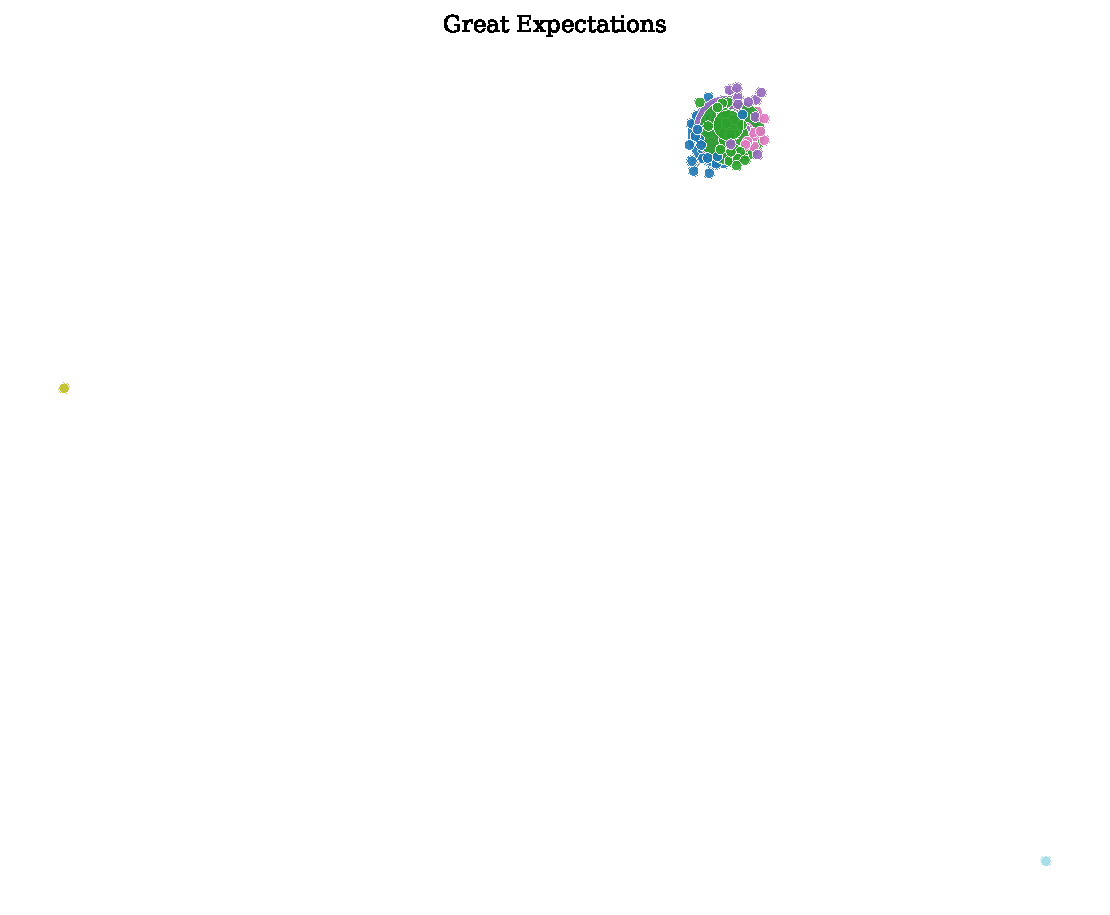
\includegraphics[width=0.74\textwidth]{figures/net_great-expectations.pdf}\caption{Character co-occurrence network of \emph{Great Expectations}. Node size is proportional to betweenness and colours denote communities (greedy modularity); the most central characters are named in the accompanying table.}\end{figure}

\begin{table}[H]\centering\small
\begin{tabular}{lrrrr}
\toprule
Character & $C_B$ & Degree & Closeness & Eigenvector \\
\midrule
Joe & 0.496 & 87 & 18.77 & 0.409 \\
Pip & 0.456 & 101 & 18.88 & 0.472 \\
Herbert & 0.449 & 84 & 18.49 & 0.258 \\
Miss Havisham & 0.228 & 74 & 18.70 & 0.427 \\
Wemmick & 0.139 & 59 & 18.21 & 0.191 \\
Mr. Jaggers & 0.098 & 63 & 18.20 & 0.239 \\
Estella & 0.066 & 70 & 18.21 & 0.325 \\
Mr. Pumblechook & 0.049 & 48 & 17.83 & 0.176 \\
Sarah Pocket & 0.032 & 28 & 16.40 & 0.076 \\
Mr. Pocket & 0.027 & 35 & 15.45 & 0.070 \\
\bottomrule
\end{tabular}
\caption{Top-10 characters in \emph{Great Expectations} ranked by betweenness.}\end{table}
\clearpage

\subsection{Huckleberry Finn (Twain, 1884)}

\begin{figure}[H]\centering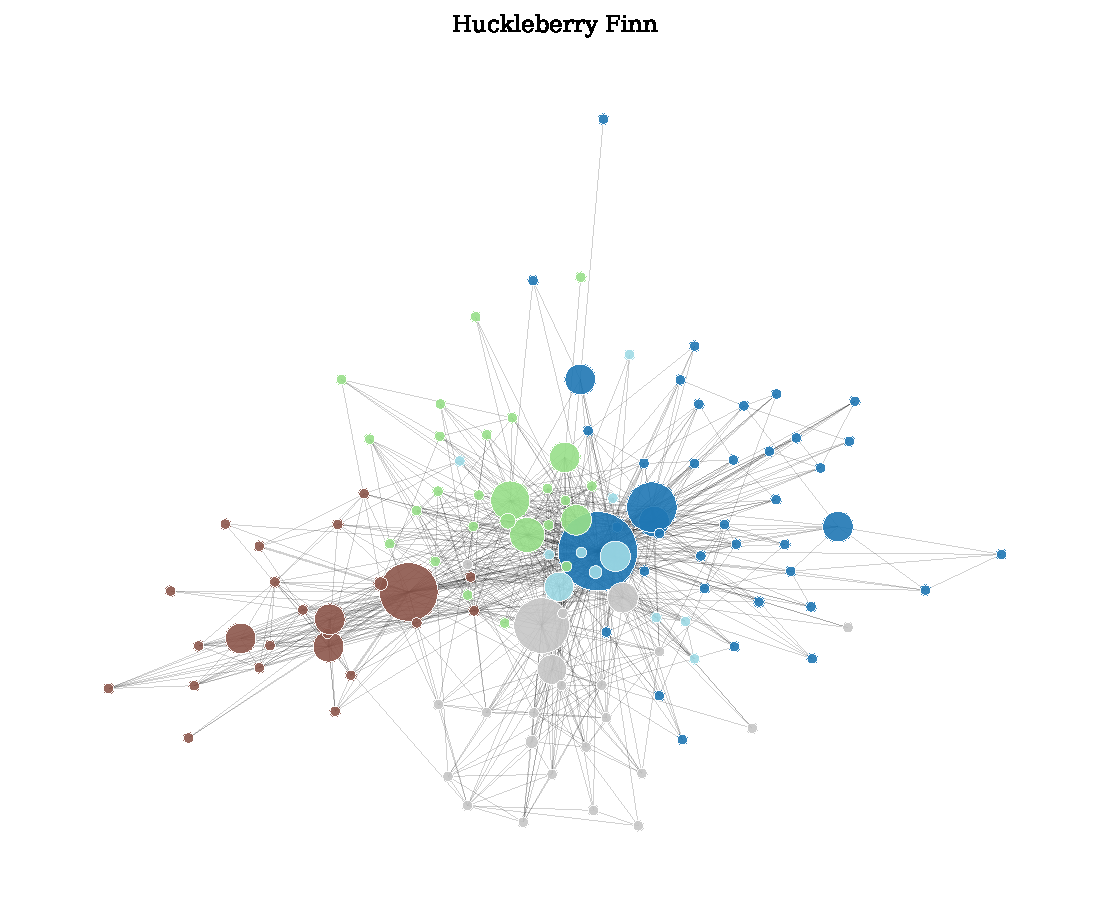
\includegraphics[width=0.74\textwidth]{figures/net_huckleberry-finn.pdf}\caption{Character co-occurrence network of \emph{Huckleberry Finn}. Node size is proportional to betweenness and colours denote communities (greedy modularity); the most central characters are named in the accompanying table.}\end{figure}

\begin{table}[H]\centering\small
\begin{tabular}{lrrrr}
\toprule
Character & $C_B$ & Degree & Closeness & Eigenvector \\
\midrule
Jim & 0.901 & 108 & 13.02 & 0.615 \\
Mary Jane & 0.263 & 49 & 10.57 & 0.088 \\
Buck & 0.211 & 46 & 11.07 & 0.109 \\
Aunt Sally & 0.140 & 44 & 12.43 & 0.358 \\
Bill & 0.048 & 35 & 9.58 & 0.075 \\
Pap & 0.029 & 42 & 11.52 & 0.161 \\
Peter & 0.017 & 26 & 8.92 & 0.023 \\
Harvey & 0.016 & 17 & 9.05 & 0.021 \\
Dey & 0.016 & 29 & 10.70 & 0.089 \\
Sherburn & 0.016 & 20 & 6.48 & 0.041 \\
\bottomrule
\end{tabular}
\caption{Top-10 characters in \emph{Huckleberry Finn} ranked by betweenness.}\end{table}
\clearpage

\subsection{The Adventures of Sherlock Holmes (Doyle, 1892)}

\begin{figure}[H]\centering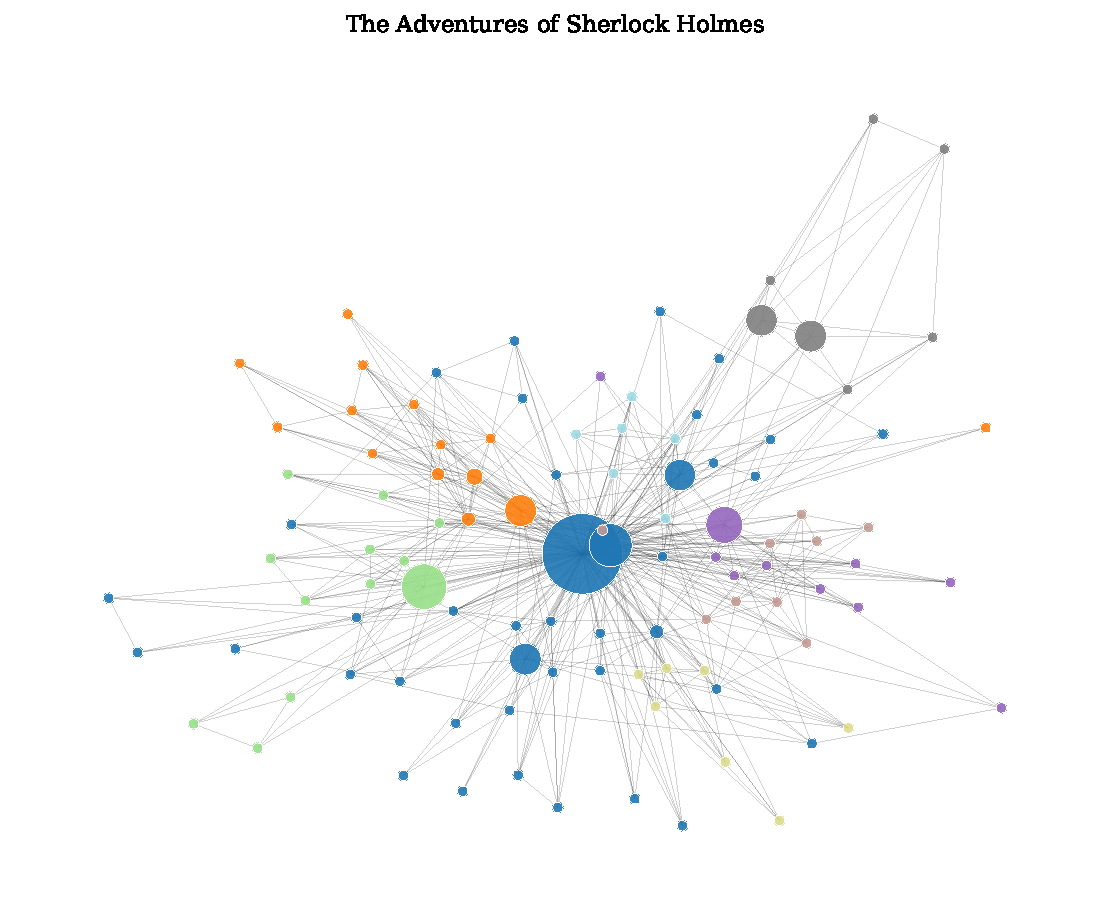
\includegraphics[width=0.74\textwidth]{figures/net_sherlock-holmes.pdf}\caption{Character co-occurrence network of \emph{The Adventures of Sherlock Holmes}. Node size is proportional to betweenness and colours denote communities (greedy modularity); the most central characters are named in the accompanying table.}\end{figure}

\begin{table}[H]\centering\small
\begin{tabular}{lrrrr}
\toprule
Character & $C_B$ & Degree & Closeness & Eigenvector \\
\midrule
Holmes & 0.971 & 102 & 18.97 & 0.655 \\
Lord St. Simon & 0.093 & 15 & 16.62 & 0.132 \\
Watson & 0.073 & 76 & 18.34 & 0.487 \\
Miss Hunter & 0.037 & 18 & 16.47 & 0.131 \\
Isa Whitney & 0.019 & 10 & 8.30 & 0.019 \\
Mr. Hatherley & 0.019 & 17 & 14.68 & 0.058 \\
Irene Adler & 0.019 & 12 & 15.62 & 0.081 \\
John Openshaw & 0.018 & 20 & 14.89 & 0.084 \\
Kate & 0.018 & 9 & 8.84 & 0.021 \\
young McCarthy & 0.001 & 16 & 16.43 & 0.134 \\
\bottomrule
\end{tabular}
\caption{Top-10 characters in \emph{The Adventures of Sherlock Holmes} ranked by betweenness.}\end{table}
\clearpage

\subsection{Emma (Austen, 1815)}

\begin{figure}[H]\centering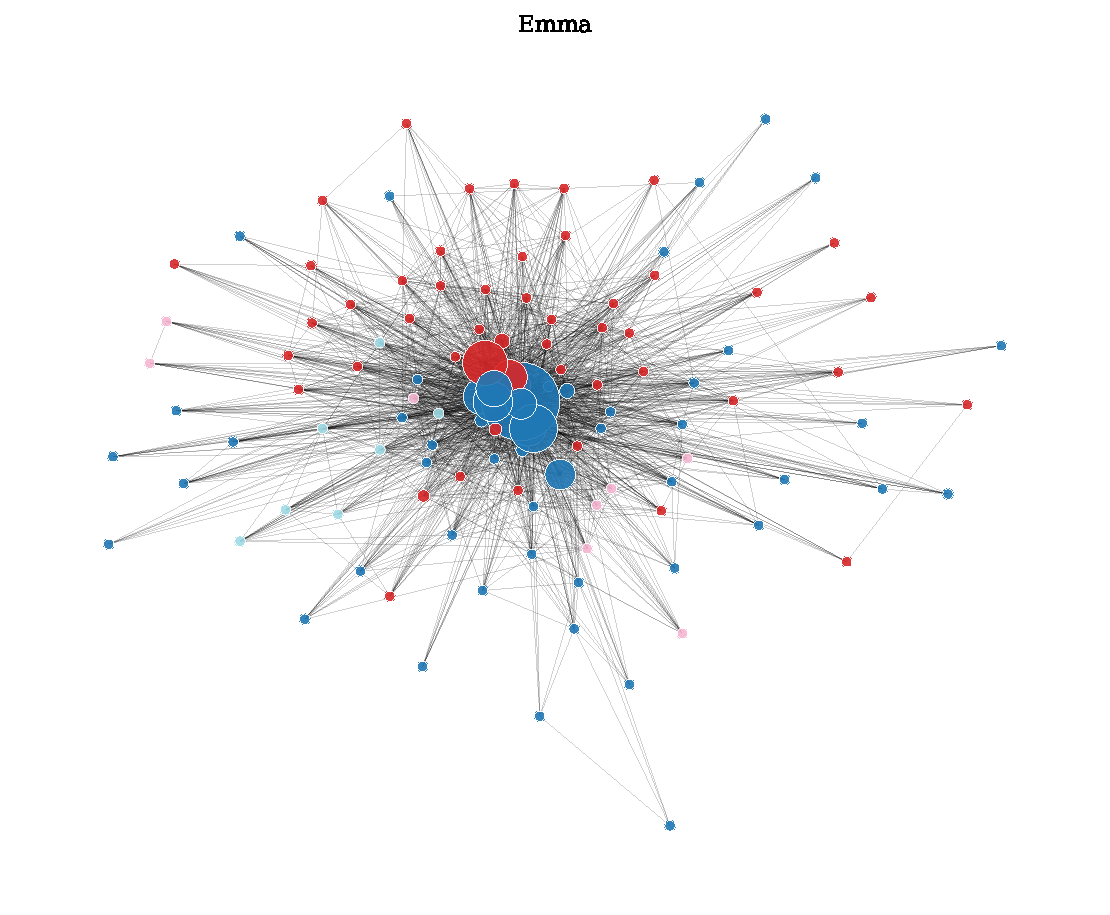
\includegraphics[width=0.74\textwidth]{figures/net_emma.pdf}\caption{Character co-occurrence network of \emph{Emma}. Node size is proportional to betweenness and colours denote communities (greedy modularity); the most central characters are named in the accompanying table.}\end{figure}

\begin{table}[H]\centering\small
\begin{tabular}{lrrrr}
\toprule
Character & $C_B$ & Degree & Closeness & Eigenvector \\
\midrule
Emma & 0.861 & 118 & 20.05 & 0.479 \\
Harriet & 0.116 & 103 & 19.78 & 0.307 \\
Mrs. Elton & 0.087 & 78 & 19.32 & 0.153 \\
Mrs. Weston & 0.051 & 95 & 19.71 & 0.299 \\
Mr. Knightley (\#281) & 0.034 & 100 & 19.76 & 0.320 \\
Mr. Weston & 0.034 & 88 & 19.54 & 0.236 \\
Mr. Elton & 0.033 & 92 & 19.55 & 0.212 \\
Miss Fairfax & 0.028 & 93 & 19.66 & 0.250 \\
Miss Woodhouse & 0.019 & 101 & 19.62 & 0.261 \\
Mr. Woodhouse & 0.017 & 103 & 19.50 & 0.220 \\
\bottomrule
\end{tabular}
\caption{Top-10 characters in \emph{Emma} ranked by betweenness.}\end{table}
\clearpage

\subsection{Jane Eyre (Brontë, 1847)}

\begin{figure}[H]\centering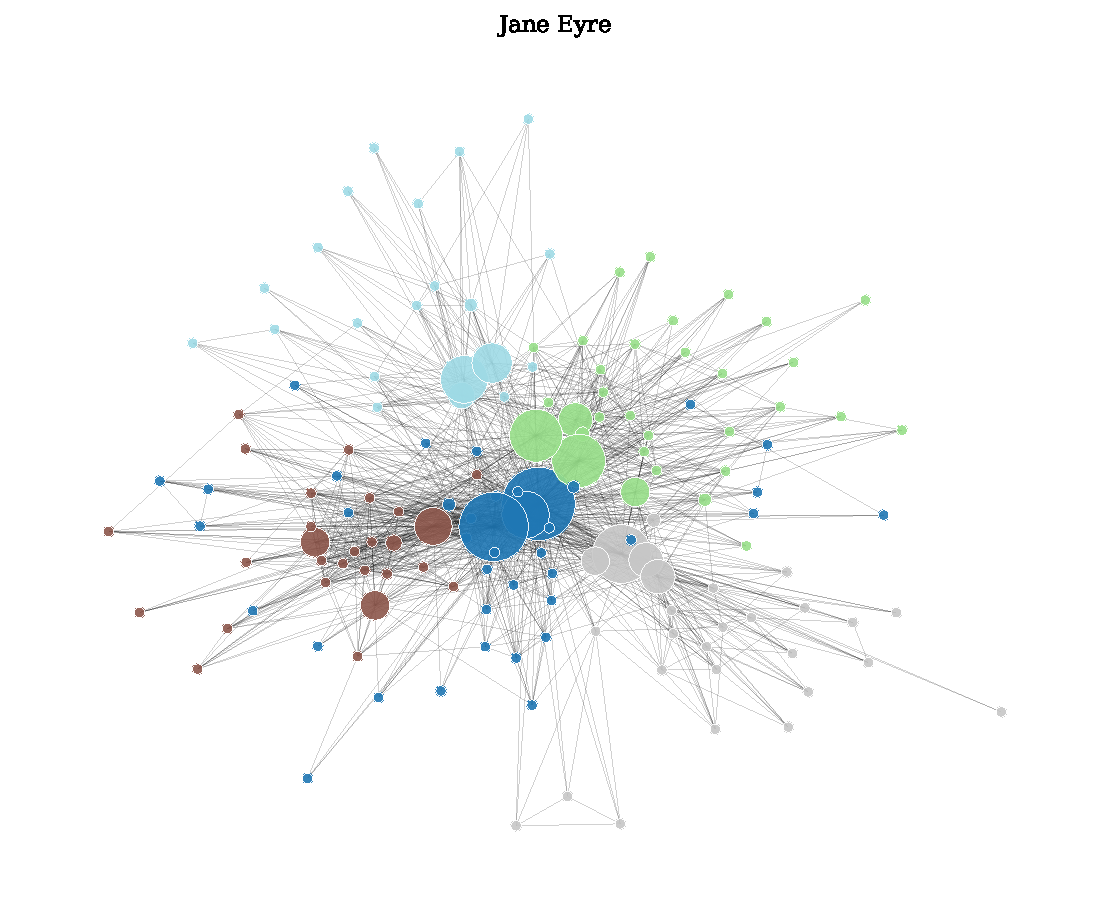
\includegraphics[width=0.74\textwidth]{figures/net_jane-eyre.pdf}\caption{Character co-occurrence network of \emph{Jane Eyre}. Node size is proportional to betweenness and colours denote communities (greedy modularity); the most central characters are named in the accompanying table.}\end{figure}

\begin{table}[H]\centering\small
\begin{tabular}{lrrrr}
\toprule
Character & $C_B$ & Degree & Closeness & Eigenvector \\
\midrule
Jane & 0.662 & 103 & 17.52 & 0.460 \\
Mr. Rochester & 0.523 & 101 & 17.42 & 0.498 \\
St. John & 0.265 & 66 & 16.81 & 0.252 \\
Bessie & 0.181 & 72 & 16.72 & 0.195 \\
Mrs. Reed & 0.171 & 65 & 16.66 & 0.139 \\
Miss Temple & 0.111 & 31 & 14.99 & 0.053 \\
Mrs. Fairfax & 0.107 & 113 & 17.30 & 0.453 \\
Helen & 0.054 & 26 & 14.85 & 0.039 \\
Miss Ingram & 0.040 & 50 & 16.24 & 0.131 \\
Mary & 0.027 & 40 & 15.99 & 0.125 \\
\bottomrule
\end{tabular}
\caption{Top-10 characters in \emph{Jane Eyre} ranked by betweenness.}\end{table}
\clearpage